% !TEX root = ../main.tex
\chapter{Przedmiot pracy}
\label{ch:przedmiot}

Rozdział ten jest poświęcony szczegółowemu opisowi przedmiotu pracy magisterskiej, którym jest system automatycznej detekcji nadużyć w komunikacji tekstowej użytkowników platformy C2C Stylify. Przedstawione zostaną założenia projektowe, uzasadnienie wyborów architektonicznych oraz szczegółowy opis implementacji poszczególnych modułów systemu.
Uzasadnia on wybory projektowe, które zostały podjęte podczas implementacji systemu detekcji nadużyć, oraz opisuje architekturę systemu i mechanizm tury konwersacyjnej, który został wprowadzony w celu skuteczniejszego wykrywania nadużyć rozbitych na wiele wiadomości. Szczególną uwagę poświęcono również implementacji Modułu D, który okazał się najlepszym podejściem do detekcji nadużyć w badaniach opisanych w rozdziale~\ref{ch:badania}.

\section{Założenia projektowe}
System detekcji nadużyć zaprojektowano z~następującymi założeniami:

\begin{itemize}
  \item \textbf{Język docelowy}: wyłącznie język polski, ze~wsparciem
    dla kolokwializmów, skrótów i~celowych błędów ortograficznych

  \item \textbf{Trzy kategorie nadużyć}: obejście systemu prowizyjnego
    platformy (\english{platform bypass}), oszustwo finansowe (\english{fraud})
    oraz toksyczność (\english{toxicity}).
  Moduł~B wykorzystuje bibliotekę Presidio \cite{bib:presidio}
    wykrywanie PII z~użyciem Presidio (B), klasyfikacja neuronowa
    opartą na~modelu HerBERT (C) oraz hybrydowy potok B~+~C~(D).

  \item \textbf{Zbiór danych}: w~fazie początkowej w~pełni syntetyczny
    (1\,200 przykładów generowanych szablonowo); wraz z~uruchomieniem
    platformy i~działaniem panelu moderatora zbiór będzie systematycznie
    wzbogacany o~realne wiadomości opatrzone etykietami moderatorów.

  \item \textbf{Integracja produkcyjna}: moduł D działa
    na~żywo jako osobny mikroserwis i~jest wywoływany przy każdej
    wysłanej wiadomości, a~jego decyzja wpływa natychmiastowo
    na~widoczność wiadomości dla odbiorcy.
\end{itemize}

\section{Uzasadnienie wyborów projektowych}

Każda istotna decyzja projektowa wynika z~analizy alternatyw i~ograniczeń
kontekstu produkcyjnego.

\paragraph{System regułowy jako punkt odniesienia (Moduł~A).}
Wdrożenie systemu regułowego jako punktu startowego uzasadnia kilka względów.
  Moduł~C to klasyfikator neuronowy oparty na~modelu HerBERT
nie wymaga danych treningowych~- co~ma~kluczowe znaczenie na~początku
projektu, gdy~anotowany zbiór jeszcze nie~istnieje. Po~drugie, system
deterministyczny pozwala na~dokładne zrozumienie jego zachowania i~stanowi
naturalny punkt bazowy (\english{baseline}) dla~porównania z~podejściami ML.
Po~trzecie, podobne systemy są~już stosowane w~praktyce przez platformy C2C
jako pierwsza linia obrony, co~czyni takie porównanie bezpośrednio użytecznym.

\paragraph{Microsoft Presidio zamiast czystego systemu regułowego (Moduł~B).}
  Moduł~D łączy Moduł~B (Presidio) i~Moduł~C (HerBERT) w~dwustopniowy
rozpoznawaczy (\english{recognizer registry}), która umożliwia łączenie wyrażeń
regularnych z~modelem językowym (spaCy) w~ramach jednego rozpoznawacza.
Słowa kontekstowe podnoszą wynik pewności~- dzięki temu fraza
\textit{,,telefon: 123 456 789''} rozpoznawana jest z~wyższą pewnością niż
sam ciąg cyfr bez~kontekstu. Alternatywa w~postaci własnych wyrażeń regularnych
byłaby funkcjonalnie równoważna dla~wzorców strukturalnych (IBAN, e-mail),
lecz~nie~rozróżniałaby kontekstu i~wymagałaby znacznie większego nakładu pracy
przy~rozbudowie o~nowe kategorie nadużyć.

  HerBERT klasyfikuje równolegle
Jako model bazowy do~dostrajania wybrano HerBERT zamiast wielojęzycznego \xlmr
z~trzech powodów. Po~pierwsze, HerBERT przetrenowany jest wyłącznie na~polskich
tekstach~- jego tokenizacja i~reprezentacje wektorowe lepiej odpowiadają
morfologii polskiej, co~przekłada się na~wyższe wyniki w~testach KLEJ
\cite{bib:herbert}. Po~drugie, monojęzyczny model jest mniejszy i~szybszy
w~inferencji niż \xlmr, co~ma~istotne znaczenie w~środowisku produkcyjnym
bez~akceleratorów GPU. Po~trzecie, dostępność przez Hugging~Face Transformers
\cite{bib:hf-transformers} i~licencja MIT zapewniają swobodę wdrożenia
bez~ograniczeń licencyjnych.

\paragraph{Hybrydowy potok zamiast jednego modelu (Moduł~D).}
Moduł~D łączy Presidio (B) i~HerBERT (C) w~kaskadzie, zamiast wybierać
jeden z~nich. Uzasadnieniem jest komplementarność błędów: Presidio jest precyzyjny
dla~wzorców strukturalnych (numery IBAN, e-mail), ale nie~rozumie semantyki;
HerBERT rozumie intencję, lecz~może przeoczyć subtelnie zasłonięty numer
telefonu. Kaskada, w~której Presidio pracuje jako szybki klasyfikator wstępny,
a~HerBERT uruchamiany jest tylko dla~wiadomości przepuszczonych przez Presidio,
łączy obie zalety przy~akceptowalnym koszcie obliczeniowym.

\paragraph{Modele LLM jako klasyfikatory zewnętrzne (podejście odrzucone).}
Alternatywą dla~opisanego potoku byłoby przesyłanie każdej wiadomości do~zewnętrznego
API dużego modelu językowego - np.\ OpenAI GPT-4 lub dedykowanego
\textit{Moderation API} \cite{bib:openai-moderation} - i~zlecanie mu
decyzji moderacyjnej. Podejście to~omówiono w~rozdziale~\ref{sec:sota}
jako jeden ze~współczesnych trendów w~dziedzinie. Zostało ono jednak
świadomie wykluczone z~niniejszej pracy z~czterech powodów.

Po~pierwsze, RODO: treści wiadomości użytkowników platformy
musiałyby być przesyłane na~serwery zewnętrznego dostawcy spoza
Europejskiego Obszaru Gospodarczego, co~rodzi poważne wątpliwości
prawne bez~jednoznacznej zgody użytkowników.
Po~drugie, koszt i~opóźnienie: wywołanie API dla~każdej
wiadomości generuje koszt proporcjonalny do~liczby tokenów oraz
opóźnienie rzędu setek milisekund - nieakceptowalne przy setkach
tysięcy wiadomości dziennie w~środowisku produkcyjnym.
Po~trzecie, niedeterministyczność: ta~sama wiadomość może
zostać oceniona inaczej przy~kolejnym wywołaniu, co~utrudnia testowanie
regresyjne i~zapewnienie spójności systemu moderacji.
Po~czwarte, brak dostrojenia domenowego: gotowe modele ogólne
nie~są~optymalizowane pod~kątem polskojęzycznego czatu marketplace,
a~frazy obejścia platformy specyficzne dla~Stylify byłyby dla~nich
nieznane bez~dodatkowego kontekstu w~zapytaniu.

Z~tych powodów zdecydowano o~budowie własnego potoku opartego
na~lokalnie wdrożonych komponentach (Presidio i~HerBERT),
który nie~wymaga transmisji danych użytkowników poza infrastrukturę
platformy.

\paragraph{Mechanizm tury konwersacyjnej.}
Klasyfikacja na~poziomie pojedynczej wiadomości jest podatna na~ataki
fragmentowane~- gdy nadawca rozkłada dane kontaktowe na~kilka krótkich
komunikatów, żaden z~nich nie~jest szkodliwy z~osobna. Tura konwersacyjna,
budowana jako ciąg kolejnych wiadomości od~tego samego nadawcy przed~odpowiedzią
drugiej strony, umożliwia wykrywanie takich ataków bez~modyfikacji modeli
klasyfikacyjnych~- wystarczy dostarczyć im~pełniejszy kontekst wejściowy.

\paragraph{Kolejność podejść jako celowy wybór metodyczny.}
Kolejność modułów A~-~D nie~jest przypadkowa. Reprezentuje rosnącą złożoność
techniczną: od~deterministycznych wyrażeń regularnych (A), przez kontekstowe
wykrywanie encji (B), po~głęboki model neuronowy (C) i~ich hybrydę (D).
Takie uszeregowanie pozwala na~obserwację przyrostu skuteczności na~każdym
kolejnym etapie i~odpowiedzenie na~pytanie, w~którym momencie dodatkowa
złożoność przestaje dawać istotny zysk. Jednocześnie każdy kolejny moduł
buduje na~poprzednim: B~zastępuje ręcznie pisane reguły A~przemyślaną
architekturą, C~wnosi rozumienie semantyczne niedostępne dla~B,
a~D~łączy mocne strony B~i~C. Wyniki tej progresji przedstawia
rozdział~\ref{ch:badania}.

\section{Architektura systemu}
\label{sec:architektura}

System składa się z~czterech głównych komponentów przedstawionych
na~rys.~\ref{fig:architektura}.

\begin{figure}[H]
\centering
\renewcommand{\arraystretch}{1.4}
\begin{tabular}{|c|}
\hline
\textbf{Interfejs użytkownika} (React) \\
Interfejs czatu użytkownika \\
\hline
\end{tabular}
\\[0.4em]
$\updownarrow$ \small{REST API / HTTP}
\\[0.4em]
\begin{tabular}{|c|}
\hline
\textbf{Część serwerowa} (Node.js / Express) \\
Moduł~A: system regułowy \quad Budowanie tury konwersacyjnej, panel moderatora \\
Moduł~D: potok hybrydowy B\,+\,C \\
\hline
\end{tabular}
\\[0.4em]
\begin{tabular}{cc}
$\downarrow$ HTTP (sieć Docker) & $\downarrow$ SQL (Sequelize) \\[0.3em]
\begin{tabular}{|c|}
\hline
\textbf{Serwis ML} (Python / FastAPI) \\
Moduł~B: \texttt{/classify/presidio} \\
Moduł~C: \texttt{/classify/herbert} \\

\hline
\end{tabular}
&
\begin{tabular}{|c|}
\hline
\textbf{Baza danych} (MySQL) \\
\texttt{Messages} \\
\texttt{MessageFlags} \\
\texttt{ConversationTurns} \\
\hline
\end{tabular}
\end{tabular}
\caption{Architektura systemu detekcji nadużyć z~zaznaczeniem modułów A-D}
\label{fig:architektura}
\end{figure}

Poszczególne komponenty pełnią następujące role:

\begin{enumerate}
  \item \textbf{Interfejs użytkownika} (React) - interfejs czatu użytkownika.
    Wysyła wiadomości do serwera i~reaguje na~zwróconą decyzję
    moderacji: wyświetla okno modalne z~ informacją o blokadzie lub baner ostrzegawczy.

  \item \textbf{Część serwerowa} (Node.js / Express) - przyjmuje wiadomości,
    buduje kontekst tury konwersacyjnej, wywołuje serwis ML i~zapisuje
    wyniki do bazy danych. Obsługuje również panel moderatora.

  \item \textbf{Serwis ML} (Python / FastAPI) - mikroserwis uruchomiony
    w~osobnym kontenerze Docker. Udostępnia punkty końcowe (\english{endpoints})
    interfejsu aplikacji \texttt{/classify/presidio} (Moduł~B) i~\texttt{/classify/herbert}
    (Moduł~C). Modele ładowane są do pamięci przy starcie kontenera.

  \item \textbf{Baza danych} (MySQL / Sequelize) - przechowuje wiadomości,
    flagi moderacji (\texttt{MessageFlags}), tury konwersacyjne
    (\texttt{ConversationTurns}) oraz decyzje moderatora.
\end{enumerate}

Środowisko uruchamiane jest przez Docker Compose, który organizuje
wszystkie kontenery i~zapewnia sieć wewnętrzną (backend komunikuje
się z~serwisem ML pod adresem \texttt{http://ml-service:8000}).

\section{Mechanizm tury konwersacyjnej}
\label{sec:tura}

Atakujący na~platformach C2C często rozbijają treści nadużycia
na~wiele krótkich wiadomości, aby ominąć detektory analizujące
pojedyncze komunikaty. Przykładem może być sekwencja:
\texttt{,,dodaj mnie''}, \texttt{,,na instagrama''}, \texttt{,,@patryk''}
- każda wiadomość z~osobna wygląda niewinnie, lecz razem stanowią
próbę wymiany danych kontaktowych poza platformą.

Aby temu zaradzić, wprowadzono pojęcie tury konwersacyjnej:
ciągu kolejnych wiadomości od~tego samego nadawcy, nieprzerwanego
odpowiedzią drugiej strony. Przed klasyfikacją każdej nowej wiadomości odpowiednia
funkcja pobiera z~bazy poprzednie wiadomości
aktualnej tury i~skleja je z~nową wiadomością w~jeden tekst kontekstowy. Granicą tury jest ostatnia wiadomość drugiego
uczestnika czatu.

Tak zbudowana tura jest przekazywana do klasyfikatorów
zamiast samej bieżącej wiadomości. Dzięki temu wykrywanie PII
(Moduł~B) i~klasyfikacja ML (Moduł~C) mają dostęp do pełnego
kontekstu nadużycia, nawet gdy zostało ono rozłożone na~kilka
wiadomości.

\section{Moduł~A: System regułowy}
\label{sec:modul-a}

Moduł~A stanowi punkt odniesienia (\english{baseline}) dla pozostałych
podejść. Implementacja opiera się na~czterech wyrażeniach regularnych i~słowniku podejrzanych
fraz:

\begin{itemize}
  \item \textbf{Wyrażenia regularne}:
    \begin{itemize}
      \item \texttt{PHONE\_REGEX} - ciągi cyfr o~długości co~najmniej
        6~znaków, z~opcjonalnym prefiksem międzynarodowym \texttt{+48}
        i~separatorami (\texttt{-}, spacja, kropka);
      \item \texttt{EMAIL\_REGEX} - adresy e-mail zgodne ze~standardem RFC~5322;
      \item \texttt{IBAN\_REGEX} - numery rachunków bankowych w~formacie
        \texttt{PL + 26 cyfr};
      \item \texttt{URL\_REGEX} - adresy URL rozpoczynające się od
        \texttt{http://} lub \texttt{https://}.
    \end{itemize}

  \item \textbf{Słownik fraz}: zestaw jedenastu wyrażeń takich jak
    \texttt{,,na priv''}, \texttt{,,zapłać poza''}, \texttt{,,nr telefonu''},
    wykrywanych metodą dopasowania podłańcucha.
\end{itemize}

Logika decyzyjna działa dwustopniowo. W~pierwszym kroku moduł sprawdza
deterministyczne reguły blokujące: wykrycie numeru telefonu zwraca
pewność obejścia 0,99; e-mail - z~pewnością 0,98; numer IBAN
- z~pewnością 0,99. W~drugim kroku, jeśli żadna reguła deterministyczna
nie zadziałała, wynik heurystyczny jest sumowany: URL dodaje~0,2,
a~podejrzana fraza -~0,4. Przekroczenie progu 0,60 skutkuje
ostrzeżeniem; poniżej progu - wiadomość jest bezpieczna.

Zaletą systemu regułowego jest deterministyczność, brak opóźnienia
i~pełna przewidywalność. Wadami są: wrażliwość na~warianty leksykalne
(celowe literówki, spacje w~numerach telefonów), brak rozumienia
semantycznego i~konieczność ręcznej rozbudowy słownika.

\section{Moduł~B: Presidio z~wyrażeniami regularnymi}
\label{sec:modul-b}

Moduł~B wykorzystuje bibliotekę Presidio \cite{bib:presidio}, otwarte narzędzie Microsoftu do~wykrywania i~anonimizacji danych
osobowych. Presidio implementuje architekturę rejestrów rozpoznawaczy
(\english{recognizer registry}), w~której każdy rozpoznawacz odpowiada
za~jeden typ encji i~może korzystać zarówno z~wyrażeń regularnych,
jak i~z~modelu NLP.

Dla potrzeb niniejszej pracy skonfigurowano dziewięć niestandardowych
rozpoznawaczy. Każdy z~nich obsługuje wyłącznie język polski i~korzysta z~modelu spaCy
\texttt{pl\_core\_news\_sm} do~przetwarzania kontekstu:

\begin{enumerate}
  \item \textbf{PHONE\_NUMBER} - trzy wzorce dla polskich numerów telefonów:
    format \texttt{+48} z~separatorami (pewność~0,95), 9~cyfr
    ze~spacjami (0,85) i~9~cyfr z~myślnikami lub bez (0,75).
    Słowa kontekstowe (,,telefon'', ,,zadzwoń'', ,,WhatsApp'')
    zwiększają wynik pewności.

  \item \textbf{IBAN\_CODE} - numery kont bankowych \texttt{PL + 26~cyfr}
    w~formacie ciągłym i~z~spacjami (pewność~0,97-0,98).

  \item \textbf{BLIK\_CODE} - 6-cyfrowe kody BLIK w~kontekście
    słów ,,blik'', ,,kod'', ,,zapłać'' (pewność~0,55).

  \item \textbf{BLIK\_REQUEST} - frazy proszące o~kod BLIK lub dane karty
    bez faktycznego numeru (np.\ ,,wyślij kod'', ,,CVV'', ,,numer karty'').
    Czternaście wzorców z~pewnością 0,80-0,95.

  \item \textbf{ADVANCE\_PAYMENT} - frazy sugerujące wyłudzenie zaliczki
    (,,zaliczka'', ,,zadatek'', ,,wpłać z~góry'', ,,przed wysyłką'').
    Dziesięć wzorców z~pewnością 0,85-0,90.

  \item \textbf{PHISHING\_LINK} - linki \texttt{http(s)://} w~kontekście
    słów ,,kliknij'', ,,zaloguj'', ,,zapłać'' (pewność~0,80).

  \item \textbf{SOCIAL\_MEDIA\_HANDLE} - trzynaście wzorców obejmujących:
    nazwy użytkownika poprzedzone \texttt{@}, bezpośrednie linki do
    Instagrama, Snapchata, Telegrama, WhatsAppa i~TikToka, skrócone
    nazwy (,,IG'', ,,FB'', ,,TT''), frazy ,,dodaj mnie na IG/FB'',
    kolokwialne formy (,,fejsa'', ,,fejsie'') oraz wzorzec
    ,,pójdźmy/przejdźmy na IG''.

  \item \textbf{BYPASS\_PHRASE} - dwadzieścia wzorców dla fraz
    obejścia platformy: ,,poza platformą'', ,,bez prowizji'',
    ,,ominąć prowizje'' (z~obsługą wariantów bez~diakrytyków),
    ,,gdzie indziej'', ,,poza Stylify'', ,,na priv''.

  \item \textbf{TOXIC\_CONTENT} - wzorce dla wulgaryzmów polskich
    i~angielskich oraz gróźb (pewność~0,80-0,85).
\end{enumerate}

Logika decyzyjna modułu jest trzystopniowa. Encje pogrupowane w~zbiorze
przy pewności $\geq 0{,}75$ skutkują zablokowaniem wiadomości. Jakakolwiek
encja z~pewnością $\geq 0{,}50$ skutkuje ostrzeżeniem. W~pozostałych
przypadkach wiadomość jest bezpieczna. Takie progi zostały dobrane eksperymentalnie.

\section{Moduł~C: Dostrojenie modelu HerBERT}
\label{sec:modul-c}

Moduł~C to klasyfikator neuronowy oparty na~modelu HerBERT
\cite{bib:herbert}, dostrojonym na~zbiorze danych własnych do~czterech
klas: \textit{bypass}, \textit{fraud}, \textit{toxic} i~\textit{benign}.

\subsection{Przygotowanie modelu}

Dostrajanie przeprowadzono w~środowisku Google Colab z~użyciem biblioteki
\texttt{Hugging Face Transformers} \cite{bib:hf-transformers}. Model bazowy
\texttt{allegro/herbert-base-cased} jest przetrenowany na~polskojęzycznych
tekstach i~cechuje się architekturą RoBERTa \cite{bib:roberta} z~tokenizacją
BPE dostosowaną do~morfologii polskiej.

Dane treningowe podzielono w~proporcji 80/10/10 (trening / walidacja / test).
Trening prowadzono przez 5~epok z~rozmiarem paczki~16 i~współczynnikiem uczenia
$2 \times 10^{-5}$. Jako funkcję kosztu zastosowano entropię krzyżową
dla czterech klas. Najlepszy punkt kontrolny (checkpoint) wybrano
na~podstawie miary~$F_1$ na~zbiorze walidacyjnym.

\subsection{Wdrożenie}

Przy starcie serwisu model ładowany jest do pamięci RAM. Odpowiedni punkt końcowy (\english{endpoint}) otrzymuje tekst do~klasyfikacji i~zwraca etykietę klasy oraz pewność.

Logika decyzyjna jest dwuprogowa: pewność \texttt{bypass} $\geq 0{,}70$ skutkuje blokadą, pewność \texttt{fraud} lub \texttt{toxic} $\geq 0{,}60$ skutkuje ostrzeżeniem, w~pozostałych przypadkach wiadomość jest bezpieczna.

\section{Moduł~D: Hybrydowy potok klasyfikacji}
\label{sec:modul-d}

Moduł~D łączy Moduł~B (Presidio) i~Moduł~C (HerBERT) w~dwustopniowy
potok, który jest aktywny w~środowisku produkcyjnym. Logika potoku
zaimplementowana po~stronie serwera Node.js. Poniżej opisano szczegóły działania każdego kroku.

\subsection{Krok 1: Presidio jako warstwa precyzji}

W~pierwszym kroku pełny tekst tury konwersacyjnej (\texttt{turnText})
jest przekazywany do modułu Presidio. Jeśli Presidio zadecyduje, że wiadomość narusza zasady, wynik jest
natychmiast zwracany do~backendu i~potok kończy działanie bez uruchamiania Modułu~C.
Uzasadnieniem tej architektury jest wysoka precyzja Presidio dla wzorców strukturalnych (numery telefonów, IBAN, kody BLIK): przypadki, w których Presidio błędnie uznaje szkodliwą treść za bezpieczną, są rzadkie dla tych kategorii. Ponadto unikanie wywołania modelu neuronowego znacznie skraca czas odpowiedzi.

\subsection{Krok 2: Podwójna klasyfikacja HerBERT}

Z kolei jeżeli Presidio nie wykryje naruszenia, tura konwersacyjna jest klasyfikowana równolegle przez dwa modele HerBERT: jeden otrzymuje bieżącą wiadomość, a drugi otrzymuje pełny tekst tury.

Podwójna klasyfikacja rozwiązuje problem rozmycia sygnału
(\english{signal dilution}): gdy tura zaczyna się od~niewinnych wiadomości,
a~nadużycie pojawia się dopiero w~ostatniej, sama bieżąca wiadomość może nie~zawierać wystarczająco silnych sygnałów dla modelu, aby ją~zaklasyfikować jako szkodliwą. Natomiast analiza całej tury pozwala modelowi uchwycić kontekst i~intencję, nawet jeśli pojedynczą wiadomość model mógłby uznać za nieszkodliwą. Klasyfikacja
samej bieżącej wiadomości zachowuje pełną siłę sygnału. Następnie wybierany jest gorszy wynik z~dwóch klasyfikacji, co~zapewnia większą czułość na~nadużycia rozłożone w~czasie.

Dla wiadomości krótszych niż cztery słowa wywołanie HerBERT jest
pomijane, co~zapobiega fałszywym alarmom na~krótkich pozdrowieniach (np.\ ,,no hejka'' - rozpoznawane
przez model jako toksyczne z~powodu przetrenowania na~krótkich tekstach).


\section{Zbiór danych}
\label{sec:dataset}

\subsection{Uzasadnienie wyboru danych syntetycznych}
\label{sec:dataset-geneza}

Budowa zbioru danych do~detekcji nadużyć w~polskojęzycznym czacie marketplace
napotyka dwie istotne bariery: brak publicznie dostępnych zbiorów dla~tej domeny
oraz przepisy RODO, które ograniczają przechowywanie i~przetwarzanie realnych
wiadomości użytkowników bez ich jednoznacznej zgody. Z~tych powodów zdecydowano
o~budowie w~pełni syntetycznego zbioru danych, wygenerowanego programistycznie.

W literaturze rozważane są trzy główne podejścia do syntetycznej augmentacji danych tekstowych. Pierwsze z nich wykorzystuje generatywne sieci przeciwstawne (Generative Adversarial Networks, GAN). Są to modele składające się z dwóch współzawodniczących ze sobą sieci neuronowych: generatora, którego zadaniem jest tworzenie nowych przykładów danych, oraz dyskryminatora, próbującego odróżnić dane wygenerowane od rzeczywistych. W wyniku tego procesu generator stopniowo uczy się tworzyć coraz bardziej realistyczne próbki. Chociaż GAN osiągnęły bardzo dobre rezultaty w generowaniu obrazów, ich bezpośrednie zastosowanie do tekstu jest utrudnione. Wynika to z dyskretnej natury tokenów językowych, która uniemożliwia bezpośrednie propagowanie gradientu przez operację \english{argmax}. Jednym z rozwiązań tego problemu jest architektura SeqGAN \cite{bib:seqgan}, wykorzystująca uczenie przez wzmacnianie do generowania sekwencji tekstowych. Jednak proces jej trenowania jest niestabilny, a w praktyce metoda ta została w dużej mierze wyparta przez nowsze podejścia.

W~niniejszej pracy wybrano podejście szablonowe, ponieważ gwarantuje
stuprocentową poprawność etykiet: każdy przykład pochodzi z~szablonu
o~z~góry określonej klasie i~nie wymaga żadnej dodatkowej weryfikacji. Podejście
jest w~pełni deterministyczne, tanie
obliczeniowo i~daje pełną kontrolę nad pokryciem wzorców w~każdej klasie.

\subsection{Schemat klas}
\label{sec:dataset-klasy}

Zbiór danych obejmuje cztery klasy odzwierciedlające kategorie zagrożeń
opisane w~rozdziale~\ref{ch:analiza}:

\begin{itemize}
  \item \textbf{bypass} (obejście platformy)~- wiadomości zawierające dane
    kontaktowe (numer telefonu w~różnych formatach, adres e-mail, nazwa konta
    w~mediach społecznościowych: Instagram, Snapchat, Telegram, WhatsApp,
    TikTok, Facebook) oraz frazy semantyczne sugerujące przeniesienie
    transakcji poza platformę bez podawania konkretnych danych
    (np.\ ,,Dogadajmy się poza serwisem'', ,,Zapłać mi bezpośrednio, po~co
    te~prowizje'').

  \item \textbf{fraud} (oszustwo finansowe)~- wiadomości wyłudzające dane
    płatnicze lub środki finansowe: prośby o~kod BLIK (z~przykładowym kodem
    lub bez), numery rachunków bankowych (IBAN) z~prośbą o~przelew, linki
    phishingowe imitujące serwisy InPost~/ Allegro~/ OLX czy żądania zaliczek
    z~góry.

  \item \textbf{toxic} (toksyczność)~- wiadomości zawierające wulgaryzmy
    i~obelgi (bezpośrednie oraz w~kontekście transakcyjnym), groźby
    (np.\ ,,Wiem gdzie mieszkasz, uważaj na~siebie''), mowę nienawiści
    i~dyskryminację grupową oraz agresywne żądania pisane z dużych liter sugerujące nieodpowiedni ton wypowiedzi.

  \item \textbf{benign} (neutralne)~- typowe wiadomości z~transakcji
    kupujący-sprzedający: pytania o~stan produktu, negocjacje ceny,
    ustalenia dotyczące wysyłki, potwierdzenia zakupu i~opinie po~transakcji.
\end{itemize}

\subsection{Metodyka generowania}
\label{sec:dataset-generowanie}

Wszystkie przykłady zostały wygenerowane skryptowo.
Dla każdej klasy przygotowano zestaw szablonów językowych z~wypełniaczami
(\english{placeholders}) zastępowanymi losowymi realistycznymi wartościami:

\begin{itemize}
  \item \textbf{numery telefonów}~- losowe numery z~polskich prefiksów
    (500-519, 600-609, 660-739, 780-791) w~sześciu formatach
    (ciągły, ze~spacjami, z~myślnikami, z~prefiksem \texttt{+48});
  \item \textbf{adresy e-mail}~- 25 wariantów nazwy użytkownika
    $\times$ 10 polskich domen (\texttt{gmail.com}, \texttt{wp.pl},
    \texttt{onet.pl} i~in.);
  \item \textbf{numery IBAN}~- format \texttt{PL} + 26 losowych cyfr;
  \item \textbf{kody BLIK}~- 6-cyfrowe liczby losowe (100\,000-999\,999);
  \item \textbf{pseudonimy} (\english{handles})~- kombinacje popularnych
    polskich imion z~liczbami, myślnikami i~kropkami;
  \item \textbf{linki phishingowe}~- fikcyjne domeny imitujące serwisy
    InPost, Allegro i~OLX z~losowym identyfikatorem ścieżki.
\end{itemize}

Bazowa pula szablonów została uzupełniona do~docelowej liczby $N = 300$
przez automatyczne tworzenie wariacji (dodanie znaku interpunkcji, prefiks
,,Hej, '' lub ,,Słuchaj, '', zmiana rejestru liter). Zabieg ten zwiększa
różnorodność stylistyczną przy zachowaniu semantycznej spójności klasy.

\subsection{Statystyki zbioru}
\label{sec:dataset-statystyki}

Tabela~\ref{tab:dataset-stats} przedstawia liczbę przykładów i~długość
wiadomości (w~słowach) w~podziale na~klasy.

\begin{table}[H]
\centering
\caption{Statystyki zbioru danych w~podziale na~klasy}
\label{tab:dataset-stats}
\renewcommand{\arraystretch}{1.2}
\begin{tabular}{lrrrr}
\hline
\textbf{Klasa} & \textbf{Liczba} & \textbf{Śr.\ słów} & \textbf{Min.} & \textbf{Maks.} \\
\hline
bypass  & 300 & 4{,}6 & 2 & 11 \\
fraud   & 300 & 5{,}9 & 2 & 11 \\
toxic   & 300 & 5{,}7 & 3 & 10 \\
benign  & 300 & 5{,}4 & 2 & 10 \\
\hline
\textbf{Łącznie} & \textbf{1\,200} & \textbf{5{,}4} & \textbf{2} & \textbf{11} \\
\hline
\end{tabular}
\end{table}

Wiadomości są krótkie (średnio 5,4~słowa), co~odpowiada rzeczywistemu
stylowi komunikacji na~platformach czatowych C2C. Wszystkie~1200 przykładów
pochodzi ze~źródła syntetycznego, więc nie zawiera żadnych danych osobowych ani wrażliwych informacji.

\subsection{Podział na~podzbiory}
\label{sec:dataset-podzial}

Zbiór podzielono losowo w~proporcji 80\,/\,10\,/\,10 na~podzbiory treningowy,
walidacyjny i~testowy. Podział przeprowadzono po~przetasowaniu
przy stałym ziarnie generatora, zapewniającym pełną
powtarzalność wyników. Podział nie~jest warstwowy:
wynikowy rozkład klas w~zbiorach walidacyjnym i~testowym nieznacznie odbiega
od~równomiernego, co~jest naturalnym efektem losowego tasowania.

Tabela~\ref{tab:dataset-split} przedstawia rozkład klas w~każdym podzbiorze.

\begin{table}[H]
\centering
\caption{Rozkład klas po~podziale na~podzbiory}
\label{tab:dataset-split}
\renewcommand{\arraystretch}{1.2}
\begin{tabular}{lrrrr}
\hline
\textbf{Klasa} & \textbf{Train (80\%)} & \textbf{Val (10\%)} & \textbf{Test (10\%)} & \textbf{Łącznie} \\
\hline
bypass  & 251 & 23 & 26 & 300 \\
fraud   & 230 & 37 & 33 & 300 \\
toxic   & 246 & 26 & 28 & 300 \\
benign  & 233 & 34 & 33 & 300 \\
\hline
\textbf{Łącznie} & \textbf{960} & \textbf{120} & \textbf{120} & \textbf{1\,200} \\
\hline
\end{tabular}
\end{table}

Różnice w~rozkładzie klas między podzbiorami są~małe (26-37 przykładów
na~klasę w~zbiorach 120-elementowych) i~nie wpływają istotnie na~reprezentatywność
oceny. Zbiór testowy jest wyłączony podczas treningu i~walidacji modeli~-
dostępny jedynie w~końcowej fazie ewaluacji wszystkich czterech podejść (A~-~D).

\section{Integracja z~platformą Stylify}
\label{sec:integracja}

\subsection{Przepływ wiadomości}

Za każdym razem, gdy użytkownik wysyła wiadomość w~systemie czatu, treść wiadomości jest analizowana jeszcze przed jej dostarczeniem do~odbiorcy. W~pierwszej kolejności system przygotowuje kontekst rozmowy, uwzględniając bieżącą wiadomość oraz wcześniejsze wiadomości należące do~tej samej tury konwersacji. Następnie nowa wiadomość zostaje zapisana w~bazie danych.

Przygotowany fragment rozmowy poddawany jest analizie przez moduł wykrywania prób oszustwa. Wynik analizy obejmuje przewidywaną kategorię zagrożenia, poziom pewności klasyfikacji oraz proponowaną akcję systemu.

Informacje o~przeprowadzonej analizie są następnie zapisywane w~bazie danych. Dla każdej wiadomości tworzony jest rekord zawierający szczegóły wykrycia, które mogą zostać wykorzystane przez moderatorów podczas dalszej weryfikacji.

W~przypadku uznania wiadomości za niebezpieczną system oznacza ją jako zablokowaną. Takie wiadomości nie są wyświetlane odbiorcy i~nie biorą udziału w~dalszej komunikacji pomiędzy użytkownikami platformy.

\subsection{Reakcja interfejsu użytkownika}

Sposób działania aplikacji po stronie użytkownika zależy od decyzji podjętej przez moduł analizy wiadomości.

\begin{itemize}
\item W~przypadku wykrycia wysokiego prawdopodobieństwa oszustwa użytkownik otrzymuje komunikat informujący o~zablokowaniu wiadomości oraz o~naruszeniu zasad korzystania z~platformy.

  \begin{figure}[h]
      \centering
      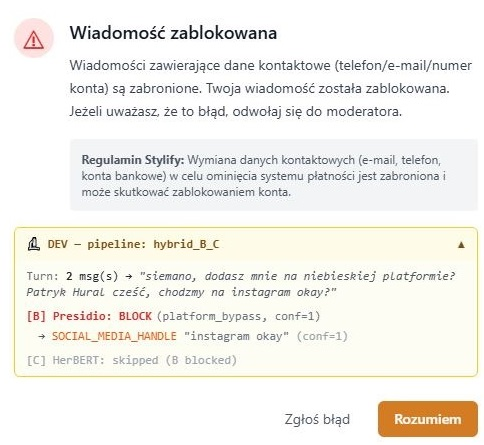
\includegraphics[width=0.5\textwidth]{block.JPG}
      \caption{Przykładowy komunikat o~blokadzie wiadomości z~interfejsu użytkownika}
      \label{fig:blockJPG}
  \end{figure}

\item Jeżeli wiadomość została uznana za potencjalnie podejrzaną, lecz poziom pewności klasyfikacji nie jest wystarczający do~jej automatycznego zablokowania, użytkownikowi wyświetlane jest ostrzeżenie zachęcające do~zachowania ostrożności.

\item Jeżeli analiza nie wykryje przesłanek wskazujących na próbę oszustwa, wiadomość zostaje dostarczona odbiorcy w~standardowy sposób.


\end{itemize}


\subsection{Panel moderatora}

Panel moderatora umożliwia przeglądanie oflagowanych wiadomości oraz weryfikację poprawności działania systemu. Moderator może sklasyfikować daną decyzję jako trafne rozpoznanie nadużycia lub jako fałszywy alarm. W~przypadku analizy zgłoszeń od~użytkowników panel pozwala również na~identyfikację pominięcia zagrożenia, czyli sytuacji, w~której system nie zareagował na~szkodliwą treść. Oznaczenie komunikatu jako fałszywy alarm automatycznie zdejmuje z~niego flagę ostrzegawczą i~przywraca mu status wiadomości bezpiecznej.

Gromadzone w~ten sposób decyzje moderatora pełnią podwójną funkcję. Po~pierwsze, stanowią wartościowe źródło danych do~ewaluacji i~dalszego treningu: każda treść zweryfikowana jako rzeczywiste nadużycie (lub zidentyfikowana jako pominięcie zagrożenia) staje się potwierdzonym przykładem ataku z~realnego ruchu komunikacyjnego. Z~kolei komunikaty sklasyfikowane jako fałszywe alarmy dostarczają systemowi sprawdzonych wzorców bezpiecznej konwersacji (klasa neutralna). Po~drugie, mechanizm ten sprawia, że~zbiór danych rośnie automatycznie wraz ze~startem platformy: im~więcej wiadomości przepływa przez system i~im~więcej decyzji weryfikuje moderator, tym więcej realnych, poprawnie opatrzonych etykietami przykładów zasila przyszłe iteracje dostrajania modelu. Docelowo etykiety nadawane w~ten sposób mogą całkowicie wyeliminować potrzebę ręcznego przygotowywania danych syntetycznych.
